\documentclass{article} % For LaTeX2e
\usepackage[final]{../colm2025_conference}

\usepackage{microtype}
\usepackage{hyperref}
\usepackage{url}
\usepackage{amsmath}
\usepackage{pifont}% http://ctan.org/pkg/pifont
\usepackage{booktabs}
\usepackage{soul}
\usepackage{cancel}
\usepackage{algorithm}
\usepackage{algpseudocode}
\usepackage{amsthm}
\usepackage{graphicx}
\usepackage{subfig}
\newtheorem{theorem}{Theorem}[section]

\usepackage{lineno}
\newcommand{\cmark}{\ding{51}}%
\newcommand{\xmark}{\ding{55}}%

\definecolor{darkblue}{rgb}{0, 0, 0.5}
\hypersetup{colorlinks=true, citecolor=darkblue, linkcolor=darkblue, urlcolor=darkblue}


\title{Week 5: Introducing Large Language Models to a General Audience}

\author{\textbf{BEH} Chuen Yang}

\newcommand{\fix}{\marginpar{FIX}}
\newcommand{\new}{\marginpar{NEW}}

\begin{document}

\ifcolmsubmission
\linenumbers
\fi

\maketitle

% https://www.youtube.com/watch?v=7xTGNNLPyMI
% Note down things you find interesting in this video lecture, organize them into a complete and self-contained report, just as you are introducing the topic to a beginner.

% \section{How To Train Your Own ChatGPT}
% - Download and preprocess the internet.
% - High quality, large diversity in documents.
%     - FineWeb is an example, 44TB of disk space.
%     - CommonCrawl -> 386TB

% - preprocess:
%     - Remove blocklisted URLs (adult, malware sites, betting sites, etc.) 
%     - Store raw HTML, then parse HTML to text.
%     - (Optionally) Remove non-English documents. (or any language you want to train on)
%     - Remove personally identifiable information (PII) such as names, addresses, phone numbers, etc.
%     - Remove duplicates.
% - Tokenize the text.
%    - Common technique is to assign numbers to represent each sequence of characters. (Possible: character, word, or sub-word tokenization)
%    - Sub-word tokenization is a good compromise between information length, and complexity.
%    - How does this encode meaning? Good analogy is emojis. 
%    - Most comon subword scheme => Byte Pair Encoding (BPE)
% - Ok, NOW you train the neural network.
%    - We simply try to predict the next token, given all **previous** tokens.
%    - Secret sauce: BACKPROPAGATION. The more educated will know this is due to the Universal Approximation Theorem.
%    - Input: Previous tokens.
%    - Output: A probability distribution over the next token.
%    - Why will it become good? We tune the parameters to be so.
%    - Motivating Philosophy: Language has causality, so we should have all the knowledge we need to predict the next token.
% - Inference
%    - Feed through the network, and sample from the probability distribution. ("Flip a biased coin")
%    - Sampling is not deterministic, so we can get different outputs for the same input.
%    - Then take the output, stick it to the back.
%    - Repeat until we reach the end of the text, or we reach a certain length.
% - Landmark paper: GPT-2
%    - This is the first time LLMs as we know them were created.
%    - Nowadays, aside from small optimizations, the architecture is more or less the same, just bigger.
% - What we end up with:
%    - A model that can blindly generate text, but may not do things like answer questions, or follow instructions.
%    - Very expensive autocomplete, uses junk from the internet.
%    - Thus pre-training is just a step one in the LLM creation process.
%    - LLMs tend to memorize things, especially base models. Karpathy gave the example of Wikipedia's Zebra page.
%        Obviously, however, they are not perfect.
%    - Where memory is not enough, the model can "hallucinate"; it generates plausible-sounding text that we know is not true.
%    - Few-shot prompting: You can coax base models into doing what you want (in-context learning), if you are smart to give it a few examples of what you want it to do.
%    - Chatbotting: Structure the prompt as though it were a conversation between a human and a robot assistant. 
%        Optionally use things like HTML tags and delineaters to make it more structured.
% - Post-training
%    - Datasets are MUCH smaller, more targeted.
%    - So where pre-training may take months, post-training may take hours only.
%    - Supervised Fine-Tuning (SFT): 
%        - For example, train on example conversations between a human and the assistant. (provided by human contractors, who follow a set of principles.)
%        - Or, train it to follow conversation rules, so it can properly structure its responses.
%        - Nowadays humans rarely write the training data, instead we use previous models to generate the training data.
%        - Mitigations for Halucinations:
%            - Explicitly tell the model that (X non-existent famous person) does not exist. (Targets the latent knowledge of the model.)
%            - Allow the model to do a "search" for information, and then use that information to answer questions. (Targets the context (i.e. "working memory"))
%        - Note that working memory tends to give better recall results than latent knowledge.
%                
%   - RL Post-Training:
%        - Analogy: In a textboook, you have the body, the examples, and the exercises.
%        - The body is the pre-trained model, the examples are the SFT, and the exercises are the RL post-training.
%        - Trial and error: Have the model generate a whole bunch of responses, and then reward the ones that are "good".
%            - Can be human feedback, can be like a compiler or somethin 
%        - Interesting tid-bits:
%            - Model reponse lengths become longer and longer.
%            - It is claimed that the model learns to "think" in a more structured way. (Actually, it is possible that these base capabilities were amplified by the RL post-training.)
%        - Taxonomy:
%            - Unverifiable results -> Reinforcement Learning from Human Feedback (RLHF) / Reinforcement Learning from AI Feedback (RLAIF)
%                - Cost-saving strat: Train a statistical model from human/AI feedback instead of directly using it.
%                - Pitfall: The model may learn to game the reward system, and produce "good" results that sound weird to the human/AI.
%            - Verifiable results -> Reinforcement Learning with Verifiable Rewards (RLVR)
% Chain of Thought (CoT):
% - What is it?
%    - A technique to improve the performance of LLMs on tasks that require reasoning.
%    - Instead of just giving the answer, the model is prompted to think step by step.
% - How does it work?
%    - We specially prompt the model to generate a sequence of reasoning steps before arriving at the final answer.
%    - So for example, Deepseek-R1 will go through what it has said, check it is all consistent/correct, before nicely formatting the final answer.
% Fantastic LLMs and where to find them:
% - Proprietary LLMs: From the likes of OpenAI (GPT-4), Anthropic (Claude), Google (Gemini), etc.
% - Open Source LLMs: From the likes of Meta (Llama 3), Deepseek (Deepseek-R1), and those who release weights on HuggingFace.
%   For bigger ones, run them on some inference providers like Hyperbolic.
%   If they are small enough, you can run them on LMStudio on your own computer.
\begin{abstract}
In this report, we summarize the salient details of "Deep Dive into LLMs like ChatGPT" by \cite{Karpathy-2025}, 
and present them in a manner suitable for a non-technical, but otherwise well-educated general audience.
It is hoped this report serves as a friendly yet insightful introduction to the topic of Language Modelling,
and conveys the important intuitions and concepts that underlie the workings of Large Language Models (LLMs) such as ChatGPT.
\end{abstract}

\section{Introduction}
Ever since GPT-3 (\cite{Brown-et-al-2020}) and ChatGPT {\cite{ChatGPT-2022}} 
first demonstrated the remarkable capabilities of Large Language Models (LLMs),
there has been a surge of interest in understanding how these models work and what they can do.
Yet as applications of LLMs transform various aspects of our daily lives,
many people still do not fully grasp the underlying principles of these models,
or how to effectively interact with them.

This report, which is overwhelmingly based on \cite{Karpathy-2025}, hopes to be a good starting point for those who wish to learn more about LLMs,
by providing a high-level overview of the key concepts and techniques involved in their development and use.

\subsection{What is an LLM?}
While there is no universally accepted definition of what an LLM is (\cite{Zhao-et-al-2023}),
a few things remain generally agreed upon \textit{in the modern context} (\cite{Zhao-et-al-2023, Sanderson-2025, Karpathy-2025}):
\begin{itemize}
    \item LLMs are \textit{neural networks} trained on massive amounts of text data in order to learn the statistical patterns of language.
    \item LLMs typically have \textit{billions or even trillions} of parameters (internal variables that the model tweaks during training).
    \item Modern LLMs typically have \textit{diverse capabilities}, (\cite{Brown-et-al-2020})
        such as generating coherent text, answering questions, following instructions, 
        and even engaging in conversations.
    \item Many modern LLMs are trained with \textit{some variant of the Transformer architecture} (\cite{Vaswani-et-al-2017}),
        which possesses a powerful attention mechanism that allows the model to determine what it should focus on in the input text.
        \footnote{
            There are some notable exceptions such as MAMBA (State Space Model) (\cite{Gu-and-Dao-2024})
            and RWKV (Recurrent Neural Network) (\cite{Peng-et-al-2023}).
            Aside from RWKV which does not suffer from the same limitations, 
            RNNs are rarely used in modern LLMs since it is difficult to parallelize them.
        }
        \footnote{
            For a great video about the Transformer architecture, see \cite{Sanderson-2025}.
        }
\end{itemize}

\section{How Do I Use LLMs?}

Perhaps the most common way to interact with LLMs is through a chat interface,
where users can type in prompts and receive responses in natural language. 
(\cite{ChatGPT-2022,Anthropic-2025,Deepseek-2024})

However, chatting is just a special case of a more general interaction paradigm,
\textit{prompt engineering} (\cite{Karpathy-2025}),
where users can provide the LLM with \textit{carefully crafted} inputs to elicit specific outputs.

Here are some common interaction techniques mentioned by \cite{Karpathy-2025}
that fall under this umbrella:
\begin{table}[h!]
\centering
\begin{tabular}{p{0.2\textwidth}p{0.8\textwidth}}
\toprule
\textbf{Technique} & \textbf{Description} \\
\midrule
\textbf{Zero-shot prompting} & Users provide a prompt without any examples,
    and the model generates a response based on its pre-trained knowledge. \\
\addlinespace
\textbf{Few-shot prompting} & Users provide a few examples of the desired input-output pairs within the prompt itself.
The model then uses these examples to generate responses that follow the same pattern. \\
\addlinespace
\textbf{Conversational prompting} & Users structure their prompts as if they are having a conversation with an AI assistant,
often using special tags or markers to distinguish between user inputs and expected assistant responses. \\
\addlinespace
\textbf{Chain of Thought (CoT) prompting (\cite{Wei-et-al-2023})} & Instead of directly asking for an answer, users prompt the model \newline 
to generate intermediate reasoning steps, which can significantly \newline 
improve performance on tasks requiring complex logical deduction. 
\\
\bottomrule
\end{tabular}
\caption{Some Prompt Engineering Techniques}
\label{tab:pe_tech}
\end{table}
\footnote{
    As \cite{Karpathy-2025} demonstrates, not affording LLMs the opportunity to think step-by-step
    within the context window (as Chain-of-Thought does) can lead to poor performance on tasks that require reasoning.
}
\footnote{
    However, you can also use LLMs in other ways, for example,
    by integrating them into applications e.g. via Anthropic's MCP (\cite{Anthropic-2025}),
    or augmenting them with external tools like ChatGPT's search functionality (\cite{ChatGPT-2022}).
}

\subsection{Where Can We Find Off-the-Shelf LLMs?}

LLMs can typically be found in four main categories: Proprietary LLMs, Open-source LLMs, Inference Providers, and Local LLMs.
Which one is the most suitable depends on the user's needs and resources.

\begin{table}[h]
\centering
\begin{tabular}{p{0.1\textwidth}p{0.9\textwidth}}
\toprule
\textbf{Type} & \textbf{Description} \\
\midrule
\textbf{Proprietary LLMs} & Among the most powerful LLMs. Developed and maintained by commercial entities, 
    such as OpenAI's GPT series (\cite{ChatGPT-2022}), Anthropic's Claude (\cite{Anthropic-2025}), 
    and Google's Gemini (\cite{Google-2025}), typically for profit. Access is typically through pay-per-token APIs. \\
\addlinespace
\textbf{Open-source LLMs} & Developed by various organizations and individuals, 
    with their underlying structures and learned weights publicly available. 
    Examples include Meta's LLaMA models (\cite{Meta-2023}) and Deepseek's models (\cite{Deepseek-2024,Deepseek-2025}). 
    Platforms like HuggingFace (\cite{Huggingface}) typically serve as repositories for these models. \\
\addlinespace
\textbf{Inference Providers} & Companies that host LLMs and provide access via APIs, 
    allowing users to run inference without needing to manage the underlying infrastructure. 
    Examples include Hyperbolic (\cite{Hyperbolic}) and other cloud-based services. \\
\addlinespace
\textbf{Local LLMs} & Smaller, open-source LLMs that can be run on personal computers 
    or local servers. Examples include Qwen3 (\cite{Alibaba-2025}). 
    These models can be run using tools like LM Studio (\cite{LMStudio}) for local inference. \\
\bottomrule
\end{tabular}
\caption{LLMs and Where to Find Them}
\label{tab:llm_types}
\end{table}

Now, let us take a closer look at how language models in general are created.\footnote{
    Note that our description considers only the seq2seq paradigm that is typically used in modern LLMs (\cite{Sutskever-et-al-2014}).
    There are other paradigms beyond the scope of this report, such as diffusion (\cite{Nie-et-al-2025}).
    \label{fn:seq2seq}
}

\section{Pre-Training: Creating a Base Model}
The key capability of an LLM is its ability to generate coherent and contextually relevant text,
which is achieved by learning the statistical patterns of language from vast amounts of text data.
This process can be achieved via \textit{self-supervised learning} (\cite{Karpathy-2025}),
where, for example, the model could learn to predict the next word in a sentence given the previous words. 

\textit{A simple analogy for this process is the act of copying a textbook in order to learn its contents.}
While arguably not very efficient for humans, this method allows the LLM to learn the structure 
and patterns of language completely from scratch.

\subsection{Data Collection \& Preprocessing}
The first step in creating an LLM is to \textit{collect and tokenize} a large corpus of text data.

In the collection stage, data is typically scoured from the Internet (due to its sheer volume and ease of access),
after which enough text is collected to fill tens of terabytes of disk space (\cite{Karpathy-2025, FineWeb-2024}).

The data is then \textit{preprocessed} (\cite{Karpathy-2025}) to ensure that it is clean, diverse, and of high quality.
A sample set of procedures is given below:
\begin{itemize}
    \item Removing URLs with a blacklist (such as \cite{UT1-2025}).
        Such URLs may contain adult content, malware, or other undesirable material.
    \item Parsing raw HTML to extract the core textual content of web pages,
        as the aim is not to learn HTML syntax but rather the human-readable contents of the website.
    \item Removing duplicate documents.
    \item Removing Personally Identifiable Information (PII) such as names and addresses.
        This is to protect the privacy of individuals whose data may have been scraped.
    \item (Optional) Filter documents to retain only specific languages if need be.
\end{itemize}

\subsection{Tokenization}
Since neural networks do not understand language symbols innately,
a natural next step is to convert text data into numbers that the model can process.
This process is called \textbf{tokenization} (\cite{Karpathy-2025}),
where the text is broken down into smaller units called "tokens." 
(To understand why we do so, see Footnote \ref{fn:seq2seq}.)

Typically, tokens are one-to-one mapping of numerical IDs to strings of symbols, as Table \ref{tab:tok_schemes} shows:
\begin{table}[h!]
\centering
\begin{tabular}{p{0.25\textwidth}p{0.5\textwidth}}
\toprule
\textbf{Tokenization Scheme} & \textbf{Symbol String} \\
\midrule
\textbf{Character-level} & Individual Characters (e.g. a, b, c) \\
\addlinespace
\textbf{Word-level} & Whole Words (e.g. "hello", "world") \\
\addlinespace
\textbf{Sub-word} & Sequences of $\geq 1$ characters (e.g. "ing", "pre") \\
\bottomrule
\end{tabular}
\caption{Tokenization Schemes}
\label{tab:tok_schemes}
\end{table}

For example, the GPT-3 model (\cite{Brown-et-al-2020}) uses a sub-word tokenization scheme 
called Byte Pair Encoding (BPE) (\cite{Sennrich-et-al-2016}), and it empirically appears to provide
a good compromise between sequence length (i.e. how many tokens are needed to represent a piece of text)
and the complexity of the model (i.e. how many "words" the model needs to learn) (\cite{Brown-et-al-2020}).

\subsection{Self-Supervised Learning}
Once the data is tokenized, the next step is to train a Transformer (\cite{Vaswani-et-al-2017}) to learn the patterns in the data.
Here, the model is trained to predict the next token in a sequence, given all the tokens that have come before it.

Practically, this means that the model ingests a sequence of tokens as input, 
processes them through its layers, and outputs a probability distribution over the next token
for each position in the sequence. See Figure \ref{fig:gpt-decoder-only} for an illustration of this process.

\begin{figure}[h]
    \centering
    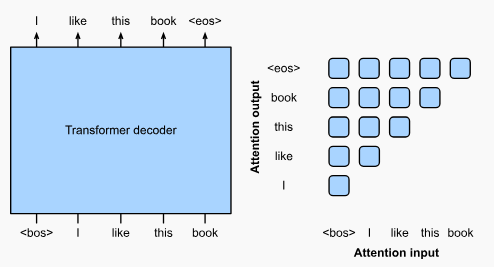
\includegraphics[width=0.8\textwidth]{images/gpt-decoder-only.png}
    \caption{How an LLM like GPT-3 processes a sequence of tokens.}
    \label{fig:gpt-decoder-only}
\end{figure}

The model is left to learn as most other neural networks do (via backpropagation) (\cite{Karpathy-2025}),
by adjusting its parameters to minimize the difference \footnote{
    This difference is usually the cross-entropy loss.
} between its predicted token probabilities and the actual next tokens
within the sequence itself.

\subsection{On The Cost of Pre-Training}
As mentioned by \cite{Karpathy-2025}, pre-training an LLM is a resource-intensive process.
Creating solid pre-trained LLMs can take months of training on powerful hardware,
often involving thousands of GPUs or TPUs working in parallel. (\cite{Alibaba-2025,Anthropic-2025,ChatGPT-2022,Deepseek-2024,Google-2025,Meta-2023})

As such, true LLM pre-training is usually the preserve of a select few immensely well-funded entities.

\subsection{Aside: Some Quirks of Base Models}
While pre-training equips an LLM with a broad understanding of whichever languages it was trained on
and a vast repository of knowledge, the base model at this point is "an extremely expensive autocomplete" (\cite{Karpathy-2025}).
It can generate text that is coherent, but as (\cite{Karpathy-2025}) notes, 
the base model, without external assistance, is not the best at generating contextually appropriate content,
following instructions, answering questions, or engaging in conversations.

While such superficial flaws can be mitigated with careful prompt engineering,
the base model still has some fundamental limitations that are worth noting.

\begin{itemize}
    \item \textbf{Latent Memory}: Base models often demonstrate a surprising ability to recall information they encounter frequently during training,
        such as the content of a well-known Wikipedia page like the one about zebras.
        This is best explained by the base model having a "latent memory" (or latent knowledge) that is burned into its parameters during pre-training.
        However, \cite{Karpathy-2025} suggests that the memorization is not infallible.
    \item \textbf{Working Memory}: Moreover, base models can utilise their context window to store
        information, retrieving them as necessary. We \textit{speculate} that this 
        is responsible for the model's ability to perform Chain of Thought (CoT) reasoning (\cite{Wei-et-al-2023}).
    \item \textbf{Hallucinations}: While base models are obviously capable of creating cogent text,
        they can inadvertently generate text that happens to be factually incorrect.
        \cite{Karpathy-2025} observes this to be the case with a fabricated person "Orson Kovacs" who does not exist in reality.
    \item \textbf{In-Context Learning}: Base models appear to have the ability to learn from the context provided in the prompt,
        which allows them to adapt their responses based on examples given, even if they have never seen those examples before,
        or if the examples are few in number ("few-shot learning").
        This is often referred to as "in-context learning" (\cite{Brown-et-al-2020}).
\end{itemize}

\section{Post-Training: Taking the Base Model Further}
In the last section, we learned that base models have limitations which limit
their usefulness in practical applications.
To address these limitations, we can take the base model and further refine it in a process known as
\textit{post-training} (\cite{Karpathy-2025}).
Most deployed LLMs today are post-trained in some way or another. (\cite{Alibaba-2025,Anthropic-2025,ChatGPT-2022,Deepseek-2024,Google-2025})

Post-training has a few traits which distinguishes it from pre-training (\cite{Karpathy-2025}):
\begin{itemize}
    \item Post-training appears to be done on a smaller, more targeted dataset,
        which is often much smaller than the dataset used for pre-training.
    \item Post-training is usually much faster than pre-training, often taking only hours instead of months.
    \item Compared to pre-training, post-training is more diverse in terms of the 
        number of techniques at practitioners' disposal to refine the LLM's behavior.
\end{itemize}

We go through the post-training techniques mentioned by \cite{Karpathy-2025} below.

\subsection{Supervised Fine-Tuning (SFT)}

In SFT, the LLM continues training as it did during pre-training,
but on a smaller dataset of high-quality examples encompassing a specific domain or task.

Sometimes, the examples are also curated to demonstrate the desired behavior of the LLM.
For example, to create a conversational AI, the LLM would be fine-tuned on a dataset of 
example dialogues between a human user and an AI assistant. Such dialogues are often
meticulously crafted by human contractors who follow detailed guidelines, but are increasingly
generated by previous iterations of LLMs to scale up the data creation process.

To continue the analogy in pre-training, \textit{
    SFT could be like providing the LLM with examples and answers from a textbook,
    whereupon it copies the examples and learns how to respond to similar questions.
}

\subsection{Reinforcement Learning (RL) Post-Training}

As mentioned at the start of this section, post-training is more diverse than pre-training. 
Indeed, SFT is not the only technique available to refine LLM behavior.
Another approach to post-training is \textbf{Reinforcement Learning (RL) post-training} (\cite{Karpathy-2025}),
which refines the LLM's behavior through maximization of a reward signal.

Again continuing the analogy from pre-training,
\textit{
    RL post-training could be like providing the LLM with exercises
    that test its understanding and application of the learned material
    from the SFT phase, allowing it to practice and improve its skills.
}

There are two main types of RL post-training (\cite{Karpathy-2025}):
\begin{itemize}
    \item \textbf{Reinforcement Learning from Human/AI Feedback (RLHF/RLAIF)}: 
        In this approach, the LLM tries to learn the most preferred responses
        based on feedback from humans or other AI systems.
    \item \textbf{Reinforcement Learning with Verifiable Rewards (RLVR)}:
        In this approach, the LLM is trained to maximize a reward signal that can be verified
        by an external system, such as an algorithm, a theorem prover, or a search engine, etc.
\end{itemize}

\subsubsection{RLHF/RLAIF}
In RLHF/RLAIF, the LLM is trained to maximize the expected reward signal from human or AI feedback.
This is typically done by generating a large number of responses to various prompts,
and then having humans or AI systems evaluate the quality of these responses.

Of course, this approach is very tough to scale up,
so it is common instead to train a statistical reward model (\cite{Zhu-et-al-2024})
which \textit{approximates} the relative rankings of responses based on human feedback,
or preferences of previously-trained LLMs.
This reward model is then used to guide the LLM's learning process,
allowing it to generate responses that are most preferred by humans or other LLMs

Naturally, the tradeoff is that the LLM may adjust itself to "game" the reward model,
by abusing imperfections in the reward model's output to generate responses that are apparently highly ranked,
but actually appear weird or nonsensical to humans or other LLMs.

\subsubsection{RLVR}
RLVR typically experiences fewer such issues as compared to RLHF/RLAIF,
in the sense that the reward signal tends to instead be rule-based, verifiable,
free of AI/human biases, and independent of statistical approximators
whose inaccuracies can be exploited by the LLM.

For example, the reward signal could be whether the code written by the LLM compiles successfully,
something which a human can use the same compiler to unambiguously double-check.

The exemplar of this approach is Deepseek-R1 (\cite{Deepseek-2024}),
which uses Group Relative Policy Optimization (GRPO) to train the LLM on math, reasoning, 
and coding tasks by verifying the correctness of the LLM's responses using a theorem prover
or a compiler.

However, this comes at the cost of flexibility, as a suitable reward signal
may not be available for every task (how do you verify that a poem is good?).

Moreover, while RLVR is verifiable, it is not \textit{infallible}.
Should there be some kind of bug in the reward signal,
the LLM may still generate responses that are inconsistent or undesirable.

\subsubsection{Another Aside: Some challenges associated with RL Post-Training}
While RL post-training is a powerful technique that can significantly improve the performance of LLMs,
it is not without challenges.

As with most RL problems (\cite{Jones-2021}), RL post-training suffers from instability due to
the multitude of moving parts within an RL post-training setup.
\footnote{
    We speculate somewhat baselessly that the high variance inherent to most RL problems 
    (\cite{Bjorck-et-al-2022, Irpan-2018})
    is mitigated somewhat by the constrained nature of the pre-trained LLM's outputs,
    which are already somewhat structured and coherent.
}

Moreover, the LLM may still be susceptible to imperfections within the RL process,
which can lead to interesting biases such as longer and longer response lengths.
(\cite{Liu-et-al-2025})

\section{Conclusion}
In this report, we have provided a beginner-friendly overview how Large Language Models (LLMs) like ChatGPT are created,
from the initial pre-training phase to the subsequent post-training phase.
We hope this document allows readers to gain a better understanding of the key concepts and techniques involved in LLM development,
and how to effectively interact with these models.

\bibliographystyle{../colm2025_conference}
\bibliography{wk5}

\appendix

\end{document}